%%%%%%%%%%%%%%%%%%%%%%%%%%%%%%%%%%%%%%%%%%%%%%%%%%%%%%%%%%%%%%%%%%%%%%
% writeLaTeX Example: A quick guide to LaTeX
%
% Source: Dave Richeson (divisbyzero.com), Dickinson College
%
% A one-size-fits-all LaTeX cheat sheet. Kept to two pages, so it
% can be printed (double-sided) on one piece of paper
%
% Feel free to distribute this example, but please keep the referral
% to divisbyzero.com
%
%%%%%%%%%%%%%%%%%%%%%%%%%%%%%%%%%%%%%%%%%%%%%%%%%%%%%%%%%%%%%%%%%%%%%%
% How to use writeLaTeX:
%
% You edit the source code here on the left, and the preview on the
% right shows you the result within a few seconds.
%
% Bookmark this page and share the URL with your co-authors. They can
% edit at the same time!
%
% You can upload figures, bibliographies, custom classes and
% styles using the files menu.
%
% If you're new to LaTeX, the wikibook is a great place to start:
% http://en.wikibooks.org/wiki/LaTeX
%
%%%%%%%%%%%%%%%%%%%%%%%%%%%%%%%%%%%%%%%%%%%%%%%%%%%%%%%%%%%%%%%%%%%%%%

\documentclass[10pt,landscape]{article}
\usepackage{amssymb,amsmath,amsthm,amsfonts}
\usepackage{multicol,multirow}
\usepackage{calc}
\usepackage{ifthen}
\usepackage[landscape]{geometry}
\usepackage[colorlinks=true,citecolor=blue,linkcolor=blue]{hyperref}
\usepackage{graphicx}
\usepackage{amsmath}


\ifthenelse{\lengthtest { \paperwidth = 11in}}
    { \geometry{top=.5in,left=.5in,right=.5in,bottom=.5in} }
	{\ifthenelse{ \lengthtest{ \paperwidth = 297mm}}
		{\geometry{top=1cm,left=1cm,right=1cm,bottom=1cm} }
		{\geometry{top=1cm,left=1cm,right=1cm,bottom=1cm} }
	}
\pagestyle{empty}
\makeatletter
\renewcommand{\section}{\@startsection{section}{1}{0mm}%
                                {-1ex plus -.5ex minus -.2ex}%
                                {0.5ex plus .2ex}%x
                                {\normalfont\large\bfseries}}
\renewcommand{\subsection}{\@startsection{subsection}{2}{0mm}%
                                {-1explus -.5ex minus -.2ex}%
                                {0.5ex plus .2ex}%
                                {\normalfont\normalsize\bfseries}}
\renewcommand{\subsubsection}{\@startsection{subsubsection}{3}{0mm}%
                                {-1ex plus -.5ex minus -.2ex}%
                                {1ex plus .2ex}%
                                {\normalfont\small\bfseries}}
\makeatother
\setcounter{secnumdepth}{0}
\setlength{\parindent}{0pt}
\setlength{\parskip}{0pt plus 0.5ex}
% -----------------------------------------------------------------------

\title{Quick Guide to LaTeX}

\begin{document}

\raggedright
\footnotesize

\begin{center}
     \Large{\textbf{A quick guide to Presentation}} \\
\end{center}
\begin{multicols}{2}
\setlength{\premulticols}{1pt}
\setlength{\postmulticols}{1pt}
\setlength{\multicolsep}{1pt}
\setlength{\columnsep}{2pt}

\subsection{Reference files}

\begin{itemize}
    \item \verb!02_presentation.text!
    \item \verb!structure_presentation.text!
\end{itemize}

\subsection{Presentation Layout Metrics}

These parameters define the layout of the presentation.

For font size:

\begin{itemize}
    \item \verb!\covertextsize!: The text size on the cover page.
    \item \verb!\titletextsize!: The title text size in each slide.
    \item \verb!\contenttextsize!: The text size in the content in each slide.
\end{itemize}

For object placement, please refer the below list and the images:

\begin{itemize}
  \item \verb!\leftmarginpos!: X value from origin to left text margin \{(0).x $\rightarrow$ (1).x\}
  \item \verb!\topmargintitle!: Y value from origin to title text (negative value!) \{(0).y $\rightarrow$ (1).y\}
  \item \verb!\topmargincontent!: Y value from origin to content text (negative value!) \{(0).y $\rightarrow$ (1).y\}
  \item \verb!\maximumwidth!: Distance value from left margin to right margin \{(3).x - (1).x\}
  \item \verb!\maximumheight!: Distance value from content top margin to bottom content margin \{(4).y - (2).y\}
  \item \verb!\columnmaxwidth!: Maximum width of content to be split 50:50 (two column presentation).
  \item \verb!\secondcolumnstart!: X value from the origin to second column. Please refer to the slide \emph{EIT Präsentation mit 2 Spalten}.
\end{itemize}

\begin{center}

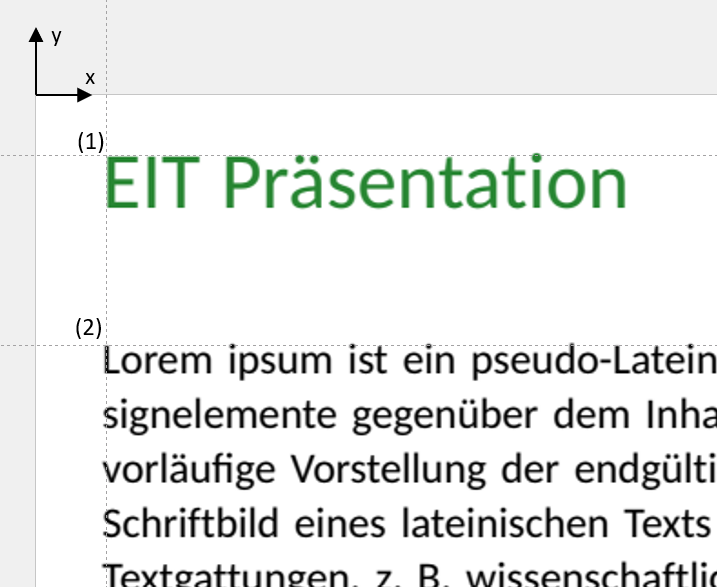
\includegraphics[scale=0.5]{Pictures/left_top_margin.png}
\end{center}
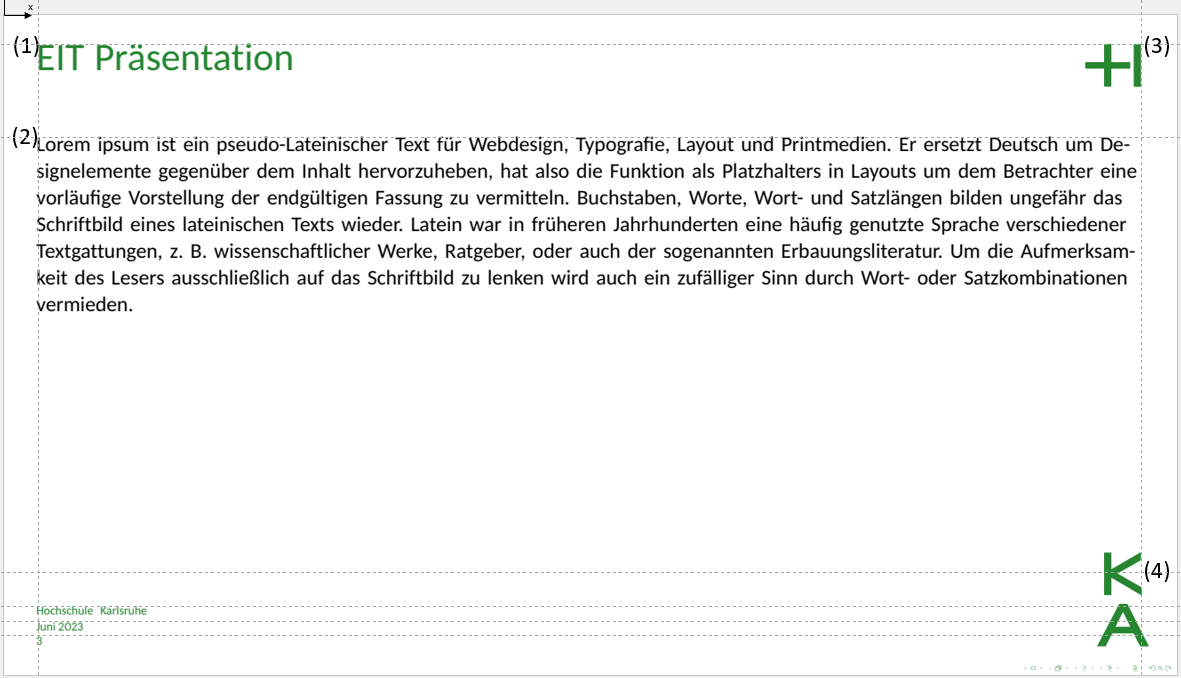
\includegraphics[scale=0.5]{Pictures/page_width_height.png}

\subsection{Helper Functions}

Positioning in presentation is done based on \textbf{tikz} and \textbf{beamer} library. There are pre-defined helper functions to quickly construct a simple presentation.

\begin{itemize}
  \item \verb!\EITCoverVI{Covert Text}{Author Name}{Picture Path}!: Create Cover Slide.
  \item \verb!\EITTableOfContent{Frame Title}{List Spacing}!: Create Table of Content slide. This slide's content is based on \verb!\section{Section Name}! defined over the document.
  \item \verb!\EITHeadlineFT{Frame Title}{Content}!: Create a normal frame. This slide's content is positioned with margins defined in layout metrics.
  \item \verb!\placetextbox{Horizontal Position}{Vertical Position}{Maximum Width}{Content}!: Override the margins to place the object in defined positions. The object anchor is at north-west (top-left) corner w.r.t the page origin.
  \item \verb!\placepictureandtext{Horizontal Position}{Vertical Position}{Maximum Width}!\\\verb!{Text Horizontal position}{Text Vertical Position}{Picture Content}{Text Content}!: Similar to \verb!\placetextbox! but
  placing picture and underlying text in defined positions. Please refer to slide \emph{EIT Präsentation mit schwebendem Bild und Text}. Should use \verb!\picdims! function for the image resize.
  \item \verb!\picdims[width=\paperwidth]{Cropped Width}{Cropped Height}{Picture Path}!: Automatically crop and trim the image w.r.t the image center following the defined dimensions. For the first optional argument, I have no idea. Just put it as shown.
  \item \verb!MeasuredFigureLabel{Figure Name}!: Replacement for figure's \verb!\label! function because of internal bug.
\end{itemize}


\end{multicols}

\end{document}
